%%%%%%%%%%%%%%%%%%%%%%%%%%%%%%%%%%%%%%%%%%%%%%%%%%%%%%%%%%%%%%%%%%%%
%%%%%%%%%%%%%%%%%%%%%%%%%%%%%%%%%%%%%%%%%%%%%%%%%%%%%%%%%%%%%%%%%%%%
%%                                                                %%
%% Esimerkki opinnäytteen tekemisestä LaTeX:lla 20130926          %%
%% Alkuperäinen versio Luis Costa,  muutokset Perttu Puska        %%
%%                                                                %%
%% Tähän esimerkkiin kuuluu tiedostot                             %%
%%               opinnaytepohja.tex (versio 1.7)                  %%
%%               aaltothesis.sty (versio 1.7)                     %%
%%               kuva1.eps                                        %%
%%               kuva2.eps                                        %%
%%                                                                %%
%%                                                                %%
%% Kääntäminen                                                    %%
%% latex:                                                         %%
%%             $ latex opinnaytepohja                             %%
%%             $ latex opinnaytepohja                             %%
%%                                                                %%
%%   Tuloksena on tiedosto opinnayte.dvi, joka                    %%
%%   muutetaan ps-muotoon seuraavasti                             %%
%%                                                                %%
%%             $ dvips opinnaytepohja -o                          %%
%%                                                                %%
%% Selittävät kommentit on tässä esimerkissä varustettu           %%
%% %%-merkeillä ja muutokset, joita käyttäjä voi tehdä,           %%
%% on varustettu %-merkeillä                                      %%
%%                                                                %%
%%%%%%%%%%%%%%%%%%%%%%%%%%%%%%%%%%%%%%%%%%%%%%%%%%%%%%%%%%%%%%%%%%%%
%%%%%%%%%%%%%%%%%%%%%%%%%%%%%%%%%%%%%%%%%%%%%%%%%%%%%%%%%%%%%%%%%%%%

%% Käytä toinen näistä, jos kirjoitat suomeksi:
%% ensimmäinen, jos käytät pdflatexia (kuvat on oltava pdf-tiedostoina)
%% toinen, jos haluat tuottaa ps-tiedostoa (käytä eps-formaattia kuville).
%%
%% Use one of these you write in Finnish:
%% the 1st when using pdflatex (use pdf figures) or
%% the 2nd when producing a ps file (use eps figures).
\documentclass[finnish,12pt,a4paper,pdftex]{article}
%\documentclass[finnish,12pt,a4paper,dvips]{article}


%% Käytä näitä, jos kirjoitat englanniksi
%%
%% Uncomment one of these if you write in English
%\documentclass[english,12pt,a4paper,pdftex]{article}
%\documentclass[english,12pt,a4paper,dvips]{article}

%% Tämä paketti on pakollinen
%% Valitse korkeakoulusi näistä: arts, biz, chem, elec, eng, sci.
%% Valiste editorisi käyttämä merkkikoodaustapa: utf8, latin1
%%
%% This package is required
%% Choose your school from arts, biz, chem, elec, eng, sci.
%% Choose the character encoding scheme used by your editor: utf8, latin1
\usepackage[sci,utf8]{aaltothesis} % this is the default in aaltothesis.sty
%\usepackage[elec,latin1]{aaltothesis}

%% Jos käytät latex-komentoa käännettäessä (oletusarvo), 
%% kuvat kannattaa tehdä eps-muotoon. Älä käytä ps-muotoisia kuvia!
%% Käytä seuraavaa latex-komennon ja eps-kuvien kanssa 
%%
%% Jos taas käytät pdflatex-komentoa, joka kääntää tekstin suoraan
%% pdf-tiedostoksi, kuvasi on oltava jpg-formaatissa tai pdf-formaatissa.
%%
%% Use this if you run pdflatex and use jpg/pdf-format pictures.
%%
\usepackage{graphicx}

%% Jos et jostain syystä pidä, miten alla oleva hyperref-paketti käyttää
%% fontteja, värejä yms., käytä tämän paketin makroja muuttamaan
%% fonttimäärittelyt. Katso paketin dokumentaatiota. Paketti määrittelee
%% \url-makron, joten ota paketti käyttöön, jos et käytä hyperref-pakettia.
%%
%% Use the macros in this package to change how the hyperref package below 
%% typesets its hypertext -- hyperlink colour, font, etc. See the package
%% documentation. It also defines the \url macro, so use the package when 
%% not using the hyperref package.
%\usepackage{url}

%% Saat pdf-tiedoston viittaukset ja linkit kuntoon seuraavalla paketilla.
%% Paketti toimii erityisen hyvin pdflatexin kanssa. 
%%
%% Use this if you want to get links and nice output with pdflatex
%%
\usepackage[pdfpagemode=None,colorlinks=true,urlcolor=red,%
linkcolor=blue,citecolor=black,pdfstartview=FitH]{hyperref}

\graphicspath{ {images/} }

\usepackage[round]{natbib}
\bibliographystyle{agsm}

%%Vaihdetaan sitaateissa and-sana ja-sanaksi
\AtBeginDocument{\renewcommand{\harvardand}{ja}}

%% Matematiikan fontteja, symboleja ja muotoiluja lisää, näitä tarvitaan usein 
%%
%% Use this if you write hard core mathematics, these are usually needed
\usepackage{amsfonts,amssymb,amsbsy}  

%% Vaakasuunnan mitat, ÄLÄ KOSKE!
\setlength{\hoffset}{-1in}
\setlength{\oddsidemargin}{35mm}
\setlength{\evensidemargin}{25mm}
\setlength{\textwidth}{15cm}
%% Pystysuunnan mitat, ÄLÄ KOSKE!
\setlength{\voffset}{-1in}
\setlength{\headsep}{7mm}
\setlength{\headheight}{1em}
\setlength{\topmargin}{25mm-\headheight-\headsep}
\setlength{\textheight}{23cm}


%% Kaikki mikä paperille tulostuu, on tämän jälkeen
%%
%% Output starts here
\begin{document}

%% Korjaa vastaamaan korkeakouluasi, jos automaattisesti asetettu nimi on 
%% virheellinen 
%%
%% Change the school field to describe your school if the autimatically 
%% set name is wrong
% \university{aalto University}{aalto-Yliopisto}
% \school{School of Science}{Perustieteiden korkeakoulu}

%% Vain kandityölle: Korjaa seuraavat vastaamaan koulutusohjelmaasi
%%
%% Only for B.Sc. thesis: Choose your degree programme. 
%%\degreeprogram{Electronics and electrical engineering}%
%%{Elektroniikka ja sähkötekniikka}
%%

%% Vain DI/M.Sc.- ja lisensiaatintyölle: valitse laitos, 
%% professuuri ja sen professuurikoodi. 
%%
%% Only for M.Sc. and Licentiate thesis: Choose your department,
%% professorship and professorship code. 
%%\department{Department of Radio Science and Technology}%
%%{Radiotieteen ja -tekniikan laitos}
\professorship{ICT Business}{ICT liiketoiminta}
\code{???}
%%

%% Valitse yksi näistä kolmesta
%%
%% Choose one of these:
%\univdegree{BSc}
\univdegree{MSc}
%\univdegree{Lic}

%% Oma nimi
%%
%% Should be self explanatory...
\author{Jaakko Lehtinen}

%% Opinnäytteen otsikko tulee vain tähän. Älä tavuta otsikkoa ja
%% vältä liian pitkää otsikkotekstiä. Jos latex ryhmittelee otsikon
%% huonosti, voit joutua pakottamaan rivinvaihdon \\ kontrollimerkillä.
%% Muista että otsikkoja ei tavuteta! 
%% Jos otsikossa on ja-sana, se ei jää rivin viimeiseksi sanaksi 
%% vaan aloittaa uuden rivin.
%% 
%% Your thesis title. If the title is very long and the latex 
%% does unsatisfactory job of breaking the lines, you will have to
%% break the lines yourself with \\ control character. 
%% Do not hyphenate titles.
\thesistitle{Thesis template}{LISÄÄ NIMI}

\place{Espoo}
%% Kandidaatintyön päivämäärä on sen esityspäivämäärä! 
%% 
%% For B.Sc. thesis use the date when you present your thesis. 
\date{KORJAA: 24.9.2013}

%% Kandidaattiseminaarin vastuuopettaja tai diplomityön valvoja.
%% Huomaa tittelissä "\" -merkki pisteen jälkeen, 
%% ennen välilyöntiä ja seuraavaa merkkijonoa. 
%% Näin tehdään, koska kyseessä ei ole lauseen loppu, jonka jälkeen tulee 
%% hieman pidempi väli vaan halutaan tavallinen väli.
%%
%% B.Sc. or M.Sc. thesis supervisor 
%% Note the "\" after the comma. This forces the following space to be 
%% a normal interword space, not the space that starts a new sentence. 
\supervisor{Prof.\ Martti Mäntylä}{Prof.\ Martti Mäntylä}

%% Kandidaatintyön ohjaaja(t) tai diplomityön ohjaaja(t)
%% 
%% B.Sc. or M.Sc. thesis advisors(s). 
%%
%% Note that there has been a change in the official EN translation
%% of the Finnish title ``ohjaaja'' which in the previous version (1.5) 
%% of this document was called ``instructor''. The recommended
%% translation is now ``advisor''.  
%% However, the LaTeX internal variable remains \instructor
%% as there is little point to change the variable name. 
%%
%\instructor{Prof. Pirjo Professori}{Prof. Pirjo Professori}
%\instructor{D.Sc.\ (Tech.) Olli Ohjaaja}{TkT Olli Ohjaaja}
\instructor{M.Sc.\ (Tech.) Tapio Jakola}{DI Tapio Jakola}

%% Aaltologo: syntaksi:
%% \uselogo{aaltoRed|aaltoBlue|aaltoYellow|aaltoGray|aaltoGrayScale}{?|!|''}
%% Logon kieli on sama kuin dokumentin kieli
%%
%% Aalto logo: syntax:
% \uselogo{aaltoRed|aaltoBlue|aaltoYellow|aaltoGray|aaltoGrayScale}{?|!|''}
%% Logo language is set to be the same as the document language.
\uselogo{aaltoRed}{''}

%% Tehdään kansilehti
%%
%% Create the coverpage
\makecoverpage


%% Suomenkielinen tiivistelmä
%% 
%% Finnish abstract
%%
%% Tiivistelmän avainsanat
\keywords{Avainsanoiksi valitaan kirjoituksen sisältöä keskeisesti kuvaavia
käsitteitä}
%% Tiivistelmän tekstiosa
\begin{abstractpage}[finnish]
  Tiivistelmässä on lyhyt selvitys (noin 100 sanaa)
  kirjoituksen tärkeimmästä sisällöstä: mitä ja miten on tutkittu,
  sekä mitä tuloksia on saatu. 
  Tiivistelmässä on lyhyt selvitys (noin 100 sanaa)
  kirjoituksen tärkeimmästä sisällöstä: mitä ja miten on tutkittu,
  sekä mitä tuloksia on saatu. 

  Tiivistelmässä on lyhyt selvitys (noin 100 sanaa)
  kirjoituksen tärkeimmästä sisällöstä: mitä ja miten on tutkittu,
  sekä mitä tuloksia on saatu. 
  Tiivistelmässä on lyhyt selvitys (noin 100 sanaa)
  kirjoituksen tärkeimmästä sisällöstä: mitä ja miten on tutkittu,
  sekä mitä tuloksia on saatu. 
  Tiivistelmässä on lyhyt selvitys (noin 100 sanaa)
  kirjoituksen tärkeimmästä sisällöstä: mitä ja miten on tutkittu,
  sekä mitä tuloksia on saatu. 
\end{abstractpage}

%% Pakotetaan uusi sivu varmuuden vuoksi, jotta 
%% mahdollinen suomenkielinen ja englanninkielinen tiivistelmä
%% eivät tule vahingossakaan samalle sivulle
%%
%% Force new page so that English abstract starts from a new page
\newpage
%
%% English abstract, uncomment if you need one. 
%% 
%% Abstract keywords
\keywords{}
%% Abstract text
\begin{abstractpage}[english]
 Your abstract in English. Try to keep the abstract short, approximately 
 100 words should be enough. Abstract explains your research topic, 
 the methods you have used, and the results you obtained.  
\end{abstractpage}
%% Note that 
%% if you are writting your master's thesis in English place the English
%% abstract first followed by the possible Finnish abstract

%% Esipuhe 
%%
%% Preface
\mysection{Esipuhe}
%\mysection{Preface}
Lisää tähän esipuhe.\\

\vspace{5cm}
Otaniemi, 24.9.2013

\vspace{5mm}
{\hfill T T.\ A.\ Teekkari \hspace{1cm}}

%% Pakotetaan varmuuden vuoksi esipuheen jälkeinen osa
%% alkamaan uudelta sivulta
%%
%% Force new page after preface
\newpage


%% Sisällysluettelo
%% 
%% Table of contents. 
\thesistableofcontents


%% Symbolit ja lyhenteet
%%
%% Symbols and abbreviations
\mysection{Käsitteet}
%\mysection{Symbols and abbreviations}




%% Sivulaskurin viilausta opinnäytteen vaatimusten mukaan:
%% Aloitetaan sivunumerointi arabialaisilla numeroilla (ja jätetään
%% leipätekstin ensimmäinen sivu tyhjäksi, 
%% ks. alla \thispagestyle{empty}).
%% Pakotetaan lisäksi ensimmäinen varsinainen tekstisivu alkamaan 
%% uudelta sivulta clearpage-komennolla. 
%% clearpage on melkein samanlainen kuin newpage, mutta 
%% flushaa myös LaTeX:n floatit 
%% 
%% Corrects the page numbering, there is no need to change these
\cleardoublepage
\storeinipagenumber
\pagenumbering{arabic}
\setcounter{page}{1}


%% Leipäteksti alkaa
%%
%% Text body begins. Note that since the text body
%% is mostly in Finnish the majority of comments are
%% also in Finnish after this point. There is no point in explaining
%% Finnish-language specific thesis conventions in English.
\section{Johdanto}
%\section{Introduction}

%% Ensimmäinen sivu tyhjäksi
%% 
%% Leave first page empty
\thispagestyle{empty}

(Tarvitsee vielä paljon hiomista ja rikastamista muista lähteistä.)

Yrityksen tulee etsiä tapoja säästää resursseja ja mahdollistaa itsepalvelu sen asiakkaille kellonajasta riippumatta, ja nämä tavoitteet ovat parhaiten saavutettavissa IT-palvelujen ja prosessessien automatisoinnilla \citep{lamoureux}. Yritykset aloittivat mekaanisen automatisoinnin jo 1950-luvulla, ja jokainen teknologinen kehitysaskel sen jälkeen on mahdollistanut yhä monimutkaisempien toimintojen automatisoinnin yrityksen toiminnassa. 

Automaatio käsitteenä sai merkityksensä autoteollisuuden tuotantolinjoilta, ja tietotekniikan yleistymisen jälkeen 1970-ja 1980-luvulla yritykset oppivat hyödyntämään automaatiota myös sisäisissä, laskentaa vaativissa prosesseissa, kuten taloushallinnossa. Internetin yleistymisen myötä 1990-2000-luvuilla teknologian kehitys on mahdollistanut liiketoimintaprosessien automatisoinnin. Koko tilaus- ja toimitusketju ja useat tuotteet ja palvelut muuttuivat digitaalisiksi. Automaatiossa ei ole siis pelkästään kysymys ihmistyön antamisesta tietokoneelle, vaan myös sen tekemisestä mikä ei aikaisemmin ollut mahdollista \citep{groover}.

Digitalisaatiosta on puhuttu jo vuosia, ja toistaiseksi se on tarkoittanut sosiaalista mediaa, mobilisaatiota, big data-analytiikkaa ja pilviteknologioiden kehitystä. Digitalisaation seuraavassa vaiheessa on kysymys ohjelmistorobotiikan ja älykkään automaation hyödyntämisestä liiketoiminnan prosesseissa. Voidaan ajatella, että seuraavan ajanjakson aikana teknologia saa aisteja, jotka olivat aikaisemmin vain ihmisen yksinoikeus \citep{groover}.

Teknologisten kehitysaskelten myötä itse teknologia muuttuu kompleksimmaksi ymmärtää, mutta niiden sovelluskohteet monipuolistuvat. Yritysten välisessä kilpailussa kyky hyödyntää uutta teknologiaa ketterästi avaa pienillekin toimijoille ovet kilpailussa jättejä vastaan. Hyvä esimerkki tästä on verkkokaupan kasvu kymmenen viime vuoden aikana. Kuluttajat ovat tottuneet saamaan haluamansa palvelut käyttöönsä yhdellä painalluksella. Sama ilmiö leviää yritysten liiketoimintaan. Odotetaan yhä isompien ja monimutkaisempien palveluiden olevan mahdollisia ottaa käyttöön hetkessä. Tämä tarjoaa pienemmille toimijoille mahdollisuuksia disruptioida markkinoita yksinkertaisella kustannustehokkaalla lähestymistavalla. Teknologinen kehitys tuo yhä monipuolisempia mahdollisuuksia kenelle tahansa luoda jotain joka ei aikaisemmin ollut mahdollista. \citep{lamoureux}

Suuryrityksillä onkin yhä enemmän paineita automatisoida prosessejaan ja investoitava uuteen teknologiaan. Puhutaan transformaatiosta, jossa olemassaolevia tietojärjestelmien määrää vähennetään, toimintoja yksinkertaistetaan,  legacy-järjestelmistä yritetään päästä eroon ja pyritään muuttamaan toimintamalli ketteräksi. Onneksi uudet teknologiat mahdollistavat tämän. Ei ole tarvetta yrittää toimia kuin start up-yritys, on tärkeämpää ymmärtää yritykselle relevantteja teknologioita ja niiden liiketoimintahyötyjä omassa kontekstissa. \citep{lamoureux}

Operaattorin näkökulmasta ilmassa on mahdollisuuksia ja uhkia. McKinseyn tekemän raportin mukaan operaattorit ovat suuressa vaarassa kärsiä disruptiosta markkinoilla. Viiden viime vuoden aikana liikevaihto alalla on ollut hitaasti laskemassa kovan hintakilpailun vuoksi, ja silti investointeja on tehtävä. Data vie koko ajan tilaa perinteisiltä tuottavilta puhe- ja viestintäpalveluilta. Operaattorit ovat vaarassa jäädä tietoliikenneyhteyksien toimittajan rooliin. Onneksi mahdollisuudetkin ovat suuret liiketoiminnan prosessien ja tarjoomien uudistuessa. Raportin mukaan yksi mahdollisuus on kehittää palveluita strategisten kumppaneiden kanssa tavalla, jossa tuotannon ja toimituksen kustannukset ovat minimoitu automatisoinnilla ja digitaalisen asiakaskokemuksen luomisella itsepalvelukanavien kautta.\citep{mckinseytele}

(Tähän parempi aasinsilta)

Asiakaspalveluratkaisujen (contact center) tarjoaminen yritysasiakkaille on ollut operaattoreiden luontaista liiketoimintaa ydinliiketoiminnan ohella. Asiakaspalvelujärjestelmät tarkoittavat yrityksen asiakkaiden yhteydenottojen käsittelemistä yhden järjestelmän kautta kanavasta riippumatta.

Operaattorit ovat olleet vahvoilla tässä liiketoiminnassa puhelinverkkojensa ansiosta. Teknologian kehittymisen myötä puhelinkanavan rinnalle on tullut muita sähköisiä kanavia, ja kanavien määrä kasvaa koko ajan sen mukaan miten asiakkaat haluavat asioida yrityksen kanssa. Kanavasta riippumatta asiakaspalvelujärjestelmän tulisi tarjota asiakaspalvelua tarjoavalle työntekijälle yksi näkymä asiakkaan tietoihin. Yrityksen järjestelmissä on erilaista tietoa asiakkaasta, joka olisi saatava helpoksi näkymäksi yrityksen työntekijälle. Asiakaspalvelujärjestelmä siis integroituu moneen eri järjestelmään ja kanavaan. Tarpeet eri integraatioille kasvavat koko ajan, koska yritykset haluavat tarjota hyvää asiakaskokemusta. Hyvään asiakaskokemukseen vaaditaan paljon tietoa eri järjestelmistä saatavilla helposti ymmärrettävässä muodossa. Asiakaspalvelujärjestelmien kehittäminen on kallista ohjelmistokehitystä, joten operaattorin on ollut helpompi tarjota valitun kumppanin tuotetta asiakkaille ja keskittyä ydinosaamiseensa, eli yhteyksien rakentamiseen asiakastoimituksissa, ja jättää itse järjestelmän kehitys kumppanille. 

Järjestelmiä tarjoavat myös muut kuin operaattorit, ja heidän kilpailuvalttinsa on ollut kustannustehokas tapa toimittaa järjestelmä, asiakaskokemus ja alhaisempi hinta. Itse puhelinkanavan merkityksen vähentyminen tarkoittaa operaattorin ainoan kilpailivaltin merkityksen vähenemistä. Näyttää siis siltä, että operaattorin asemaa asiakaspalvelujärjestelmä-markkinalla disruptoidaan. 

Tässä työssä keskitytään tarkastelemaan
Telia Finland Oyj:n asiakaspalvelujärjestelmää Kontakti L, jolle on asetettu tavoitteeksi automaattinen asiakasprosessi (tilauksen, toimituksen ja laskutuksen osalta), itsepalvelun lisääminen ja kustannustehokkuus. Kyseisellä tuotealueella ei ole aikaisemmin onnistuttu luomaan automaattista asiakasprosessia nykyisissä olosuhteissa. Tarvitaan siis selvitys siitä miten olosuhteiden tulisi muuttua automaattista asiakasprosessia varten.

\subsection{Tutkimuskysymys ja alakysymykset}

Pääkysymys: Tulee varmaankin muuttaa.
Miten asiakasprosessi tulisi rakentaa, että se vastaisi liiketoiminnan tavoitteisiin, eli nopeampiin toimituksiin, asiakastyytyväisyyden parantumiseen, kustannustehokkuuteen, nopeampiin toimintojen lanseerauksiin, mahdollistaisi experimentation and learning in the market place?
Telian täytyy psytyä rakentamaan näiden tuotteiden prosessiin nopeampi uusien teknologioiden kokeilu kuten uudet kanavat  yms. Niitä pitää saada nopeammin asiakkaille!!! Kuvaat miten paljon muutosvoimia tulossa yms ja sitten mites näihin päästään. Noh DevOps ne tuo. Mites DevOps onnistuu nykytilanteessa ja mitä pitää tehdä että sinn päästään?

Se Sofigaten liiketoimintavalmiushomma. Kuvaa nykytila, ja tavoitetila. Mikä estää matkan tavoiteltilaan? 
Mitkä osat asiakasprosessista on kannattava automatisoida?
Telian digitaalisen vision mukaan, onko 80-prosentin automatisaatioaste mahdollista saavuttaa Kontakti L:n asiakasprosessissa?

Mitkä tekijät rajoittavat asiakasprosessin automatisointia?
Miten Kontakti L:n asiakasprosessin tulisi rakentaa Miten asiakaspalvelujärjestelmän asiakasprosessissa voidaan hyödyntää.
Miten Kontakti L:n asiakasprosessi tulee rakentaa, kun siltä odotetaan toimitusvarmuutta, kustannustehokkuutta ja automatisointia.
\begin{itemize}
\item[--]Kysymys 1: Mitkä ovat ne olosuhteet, joissa Kontakti L- asiakaspalvelujärjestelmän asiakasprosessi voidaan automatisoida?
\item[--]Vastaus 1: Kuvaus automatisoidusta asiakasprosessista ja sen vaatimista olosuhteista.
\end{itemize}

Alakysymykset:
\begin{itemize}
\item[--]Kysymys 2: Mitkä ovat ne edellytykset joiden perusteella Kontakti L- asiakaspalvelujärjestelmä on kannattava tarjota digitaalisen itsepalvelukanavan kautta?
\item[--]Vastaus 2: Edellytykset digitaalisen itsepalvelukanavan hyödyntämiselle.
\item[--]Kysymys 3: Missä kohdin automatisoitua asiakasprosessia olisi järkevä hyödyntää robotiikkaa tai älykästä automaatiota?
\item[--]Vastaus 3: Asiakasprosessin vaiheet, joissa robotiikan tai älykkään automaation käyttö on perusteltua.

\end{itemize}
\subsection{Työn rakenne}
Taustatieto kappaleessa kerron yleisesti asiakasprosessista ja mitä sen automatisoinnilla voidaan saavuttaa. Kappaleessa tuodaan myös esille automaation tämän hetken trendejä. Kappale määrittää työn keskeisen konseptin.

Asiakaspalvelujärjestelmät-kappeleessa kuvataan tarkemmin minkälaisestä järjestelmästä on kysymys, eli kuvataan liiketoiminnan ongelma, jonka järjestelmä ratkaisee eri kokoisissa yrityksissä. Kappaleessa tuodaan myös esille minkälaisia järjestelmät ovat luonteeltaan ja minkälaisia tulevaisuuden trendejä on nähtävissä.

Digitaalinen visio-kappaleessa keskitytään antamaan kuva siitä minkälaisia haasteita digitalisaatio ja automatisaatio tuottavat operaattorille, ja miten näitä haasteita on alettu ratkaisemaan.

Yhteenvedossa tuodaan kappaleiden aiheet yhteen ja perustellaan miksi on olennaista tarkastella asiakasjärjestelmän asiakasprosessin automatisointia juuri Telialla.

\subsection{Tutkimuksen rajaus}


%% Opinnäytteessä jokainen osa alkaa uudelta sivulta, joten \clearpage
%%
%% In a thesis, every section starts a new page, hence \clearpage
\clearpage

\section{Taustatieto}



% \section{Background}
\subsection{Asiakasprosessi ja sen automatisoinnin arvo}

 Ohjelmistoja ja järjestelmiä tuottavien yritysten liiketoiminnan ydinprosesseihin kuuluu asiakasprosessi, eli prosessi jonka avulla asiakas ostaa ja saa käyttöön haluamansa palvelun tai tuotteen. Yrityksissä prosessit antavat viitekehyksen tavoitteiden saavuttamiseksi, jotka ovat tiukasti sidoksissa asiakasarvon luomiseen. Ohjemistotuotannon prosesseissa on aina useita ihmisiä, jotka suorittavat tehtäviä järjestelmien ja työkalujen avulla. Ihmisten yhteistyötä tehtävien suorittamiseksi ohjaavat menetelmät ja muut kontekstiin liittyvät prosessit. \citep{okaytannot}

Ihmisille on aina ollut tyypillistä luoda työkaluja työnsä helpottamiseksi, ja käytäntö antaa oppia miten työkalua tulisi parantaa entisestään \citep{groover}. Monimutkaisessa yhä useampia ihmisiä vaativissa toimenpiteissä tarvitaan määriteltyjä työkaluja yhteistyölle, eli tapoja toimia yhteisen tavoitteen saavuttamiseksi. Sen vuoksi toimintatavat on kannattava määritellä prosesseiksi, koska tällöin voidaan standartisoida systemaattinen tapa saavuttaa päämäärä. Prosessien määrittelemisen ja kuvaamisen avulla on myös mahdollista nähdä tarkemmin miten toimintatapoja tulisi kehittää, ja käyttää toimintatapoja ilman sidoksia yksilöihin.

Se mikä on sopiva tapa ja tarkkuus määrittää prosessi vaihtelee tapauskohtaisesti ja on riippuvainen sovelluskohteesta. Liian korkealla tasolla kuvattu prosessi ei välttämättä ohjaa tekemistä tarpeeksi laatutavoitetta kohden, ja liian tarkasti määritetty prosessi ohjaa tekemistä liikaa, jolloin toiminta on kankeaa. Usein vähäisemmän kokemuksen omaava ryhmä tarvitsee tarkemman rakenteen toiminnalle kuin pidemmän kokemuksen omaava ryhmä. Olennaista kuitenkin on selkeästi määritetty tavoite, jonka saavuttamista on mahdollista seurata prosessin aikana ja jälkeen. \citep{ohjelmistotuotanto}

Lähes jokaisessa yrityksessä liiketoiminta on riippuvainen tietojärjestelmistä ja niiden kehittämisestä liiketoimintavalmiuksien kasvattamiseksi. Prosessijohtamisen näkökulmasta haaste on tehdä näkyväksi tietojärjestelmiin liittyvät työprosessit. Tämä korostuu erityisesti ohjelmistotuotannon laadun johtamisessa. Perinteisessä teollisuudessa liiketoimintaprosessiin liittyvien työprosessien hallinta on viety hyvinkin pitkälle esimerkiksi Toyota Kata-filosofian edistysaskelien kautta. Liiketoimintaprosesseihin on näin pystytty rakentamaan laatu, turvallisuus ja ketteryys sisälle. 

-Asiakasprosessin automatisoinnista jotain.
-näkymättömyys

\subsubsection{Asiakasprosessi on liiketoimintaprosessi}

Liiketoimintaprosessit on yrityksen kehittämiä työkaluja sen tavoitteiden saavuttamiseksi. Yrityksen tavoite on ratkaista sen asiakkailla oleva ongelma ja tuottaa ongelman ratkaisemalla lisäarvoa \citep{teollisuustalous}. Tämän vuoksi esimerkiksi ohjelmistotuotannossa liiketoiminnan ydinprosessia, jonka avulla ratkaistaan asiakkaan ongelma, kutsutaan asiakasprosessiksi.

Liiketoimintaprosessit ovat yrityksen systemaattiset ja standartoidut työkalut niiden tavoitteiden saavuttamiseksi, jonka vuoksi yritys on olemassa. Yrityksen liiketoimintaprosessien voidaan ajatella liikkuvan horisontaalisesti sen eri toimintojen, kuten myynnin, toimituksen tai vaikkapa laskutuksen läpi. Näitä jokaiselta yritykseltä löytyviä toimintoja kutsutaan usein vertikaaleiksi. Suoraan ulkoiselle asiakkaalle arvoa tuottavia prosesseja kutsutaan liiketoiminnan ydinprosesseiksi. Liiketoimintaprosessien turvaamiseksi on olemassa tukiprosesseja sisäistä asiakasta varten, kuten esimerkiksi sisäisen tietojärjestelmän ylläpitoprosessi tai vaikkapa sisäisen viestinnän prosessi. Liiketoiminnan tukiprosessit eivät välttämättä tuota ydinprosesseihin verrattavaa arvoa, mutta kun ne lakkaavat toimimasta, niillä on huomattavia vaikutuksia yrityksen toimintaan. On huomattava, että liiketoimintaprosessilla on aina asiakas (joko sisäinen tai ulkoinen), joka saavuttaa prosessin avulla haluamansa lopputuloksen. Liiketoimintaprosessi siis ylittää organisaation rajat ja sillä on usein vähän riippuvuutta itse organisaation rakenteeseen.

Yrityksen eri toiminnoista koostuvaa prosessinäkymää kutsutaan Lean-ajattelussa arvovirraksi \citep{leanit}. Lean-ajattelussa tavoitellaan näkyvää arvotuotannon järjestelmää ja alajärjestelmiä, jolloin huomio keskitetään arvoa tuottamattomien vaiheiden poistamiseen. Orzenin ja Paderin mukaan arvovirta muokkaa syötteitä lopputuotokseksi arvotuotannon järjestelmän prosessien avulla, ja nämä prosessit vaativat resurssien hankkimista ja kuluttamista. Tyypillisiä yrityksen resursseja ovat esimerkiksi aika, raha, raaka-aineet ja työvoima. Se miten yritys päättää järjestää arvoketjun toiminnot ja hallita sitä, määrittävät tuotannosta aiheutuvat kustannukset ja tuotot. Tehokas arvovirta kuluttaa mahdollisimman vähän resursseja parhaan mahdollisen lopputuloksen aikaansaamiseksi. Toimiva arvovirta tuottaa myös aina samaa laatua joka on mitattavissa.

Laadulla ei tarkoiteta ekplisiittisesti hyvää laatua, vaan kontrolloitua laatua valittujen mittareiden perusteella \citep{okaytannot}. Kilpailussa markkinoilla korostuu yrityksen valitsemat laatutekijät, koska tuotteiden ja palveluiden laatu rakentuu toimintaprosessien laadusta \citep{ohjelmistotuotanto, teollisuustalous}. Tämän periaatteen mukaan laatua ei voi myöskään lisätä asiakasprosessilla toimitettavaan tuotteeseen tai palveluun jälkikäteen, vaan prosessi täytyy rakentaa valittujen laatutekijöiden perusteella. Laatutekijät valitaan mittaamaan liiketoiminnan tavoitteiden toteutumista. Esimerkiksi laadun asiakaslähtöinen määrittely antaa laadulle määrityksen joka mitataan asiakastarpeiden täyttämisessä onnistumisella (Sofigate). Määritelmä laadusta antaa periaatteen miten arvotuotannon toimintaa johdetaan ja kehitetään. 

Yrityksen valmiuksia parempaan ja tuottavampaan liiketoimintaan voidaan parantaa liiketoimintaprosesseja kehittämällä \citep{teollisuustalous, leanit, ohjelmistotuotanto}. Prosessien kehittämisen tulisi olla jatkuvaa, ja se usein vaatii pienten askelten ottamista kerrallaan, koska muutoksilla saattaa olla hetkellinen tuottavuutta laskeva vaikutus. Sanotaankin, että prosessien kehittämisessä onnistuminen vaatii ensisijaisesti johdon sitoutumista tukea muutosta, eli käytönnössä aikaa ja resursseja ottaa uusi prosessi käyttöön \citep{okaytannot}.

Prosessien kehittämisen edellytyksenä on prosessikulttuurin olemassaolo, jolloin voidaan olettaa toiminnan perustuvan prosessien käyttöön, mittaamiseen ja niiden avulla johtamiseen. Ilman prosessikulttuuria olisikin keskityttävä prosessikulttuurin luomiseen riittävissä määrin. Vain paperilla olevia prosesseja on turha kehittää, koska niillä ei ole yhteyttä lisäarvon tuottamiseen. \citep{teollisuustalous}

Ideana liiketoimintaprosessien kehittämisessä joko vähentää resurssien käyttöä ja eliminoida tarpeettomia työvaiheita saman lopputuloksen saavuttamiseksi, tai onnistua löytämään uusia tapoja tuottaa asiakkaalle arvoa prosessin avulla. Digitaalisten palveluiden myötä avainasemassa on uusien palvelukonseptien kehittäminen ulkoisten sidosryhmien tarpeiden mukaan, jolloin sisäisten ja ulkoisten liiketoimintaprosessien oletetaan taipuvan nopeampiin muutoksen sykleihin. Tällöin liiketoimintaprosessien kehittämisen tulee olla jatkuvaa toimintaa. (Sofigate) 

Liiketoimintaprosessien kehittämisen lähtökohtana on ymmärrys nykytilasta, tavoitetilasta ja näiden kahden tilan erojen tunnistamisesta. Näin pystytään priorisoimaan kehitystä vaativat osa-alueet. Ymmärrys nykytilasta sisältää ongelmakohtien ja tarpeettomien työvaiheiden kuvaamisen, jotka tulee poistaa tai tehostaa esimerkiksi automatisoimalla. Ymmärrys tavoitetilasta kuvaa uusia valmiuksia liiketoimintaprosessissa, joiden perusteella määritetään toiminnot, jotka tuovat tavoitteen vaatiman arvon. Nykyaikaisessa liiketoiminnassa korostuu ketterät toiminnot, jotka mahdollistavat uuden arvon luomisen nopeammin ja yksinkertaisemmin. (Sofigate)

Ymmärrys nykytilasta on helppo saavuttaa kun prosessin aktivitetit ovat näkyvillä, jolloin jokaisella toiminnolla on laatua mittaava komponentti \citep{ohjelmistotuotanto}. Tällöin prosessin tavoitten toteutumista voidaan seurata prosessin eri vaiheissa. Näin prosessin omistaja, joka on vastuussa kehittämisestä, huomaa poikkeamat ja voi parantaa ohjeistusta. Usein heikko ymmärrys nykytilasta on suurin este prosessin kehittämisessä, koska laatupoikkeamat havaitaan liian kaukana niiden alkuperäisestä aiheuttajasta \citep{teollisuustalous}.

\subsubsection{Asiakasprosessi ohjelmistotuotannossa}

Kuten aikaisemmin maninittiin (Tuotantotalous, Ohjelmistotuotanto), yrityksen työprosesseista muodostuu laatujärjestelmä, jonka mukaan pyritään laatutavoitteisiin. (Ohjelmistotuotanto, DevOps handbook) Ohjelmistotuotannossa laatujärjestelmän rooli korostuu erityisesti sen vuoksi, koska työprosessien toiminta on suurilta osin näkymätöntä, eikä laatua voi lisätä ohjelmistoihin tai järjestelmiin jälkikäteen. Tämän vuoksi laatua mittaava komponentti on oltava sisäänrakennettuna työprosessin vaiheisiin. Tehtäessä ohjelmistoja korostuukin hyvät toimintatavat, jotka on määritetty riittävän tarkasti tuottamaan tavoitteen mukaista laatua. Haaste onkin tehdä näkymättömistä työprosessin vaiheista riittävän näkyviä, jolloin prosessin eri vaiheita voidaan seurata ja arvioida niiden tehokkuutta. 

Ohjelmistotuotannon ydinprosesseihin kuuluu asiakasprosessi, tuotekehitysprosessi ja ylläpitoprosessi. Liiketoimintamalli vaikuttaa oleellisesti miten nämä prosessit tukevat toisiaan. Asiakasprosessin osalta on kolme liiketoimintamallia, täysin asiakkaan tarpeiden pohjalta rakennettava ohjelmisto tai suoraan "hyllyltä" asiakkaalle myytävä ohjelmistotuote tai palvelu. Näiden kahden ääripään välimaastossa on niin kutsuttuihin ohjelmistoalustoihin tai ekosysteemeihin perustuva malli, jossa asiakkaalle paketoidaan ohjelmistotuote tai palvelu olemassaolevista ja räätälöidyistä komponenteista. Koko ohjelmistotuotantoprosessi voidaan myös nähdä yhtenä asiakasprosessina, johon tuotekehitys ja ylläpito kuuluvat. Kuvassa \ref{fig:asiakasprosessi} on kuvattu asiakasprosessit eri liiketoimintamalleissa.

\begin{figure}[!h]
    \centering
    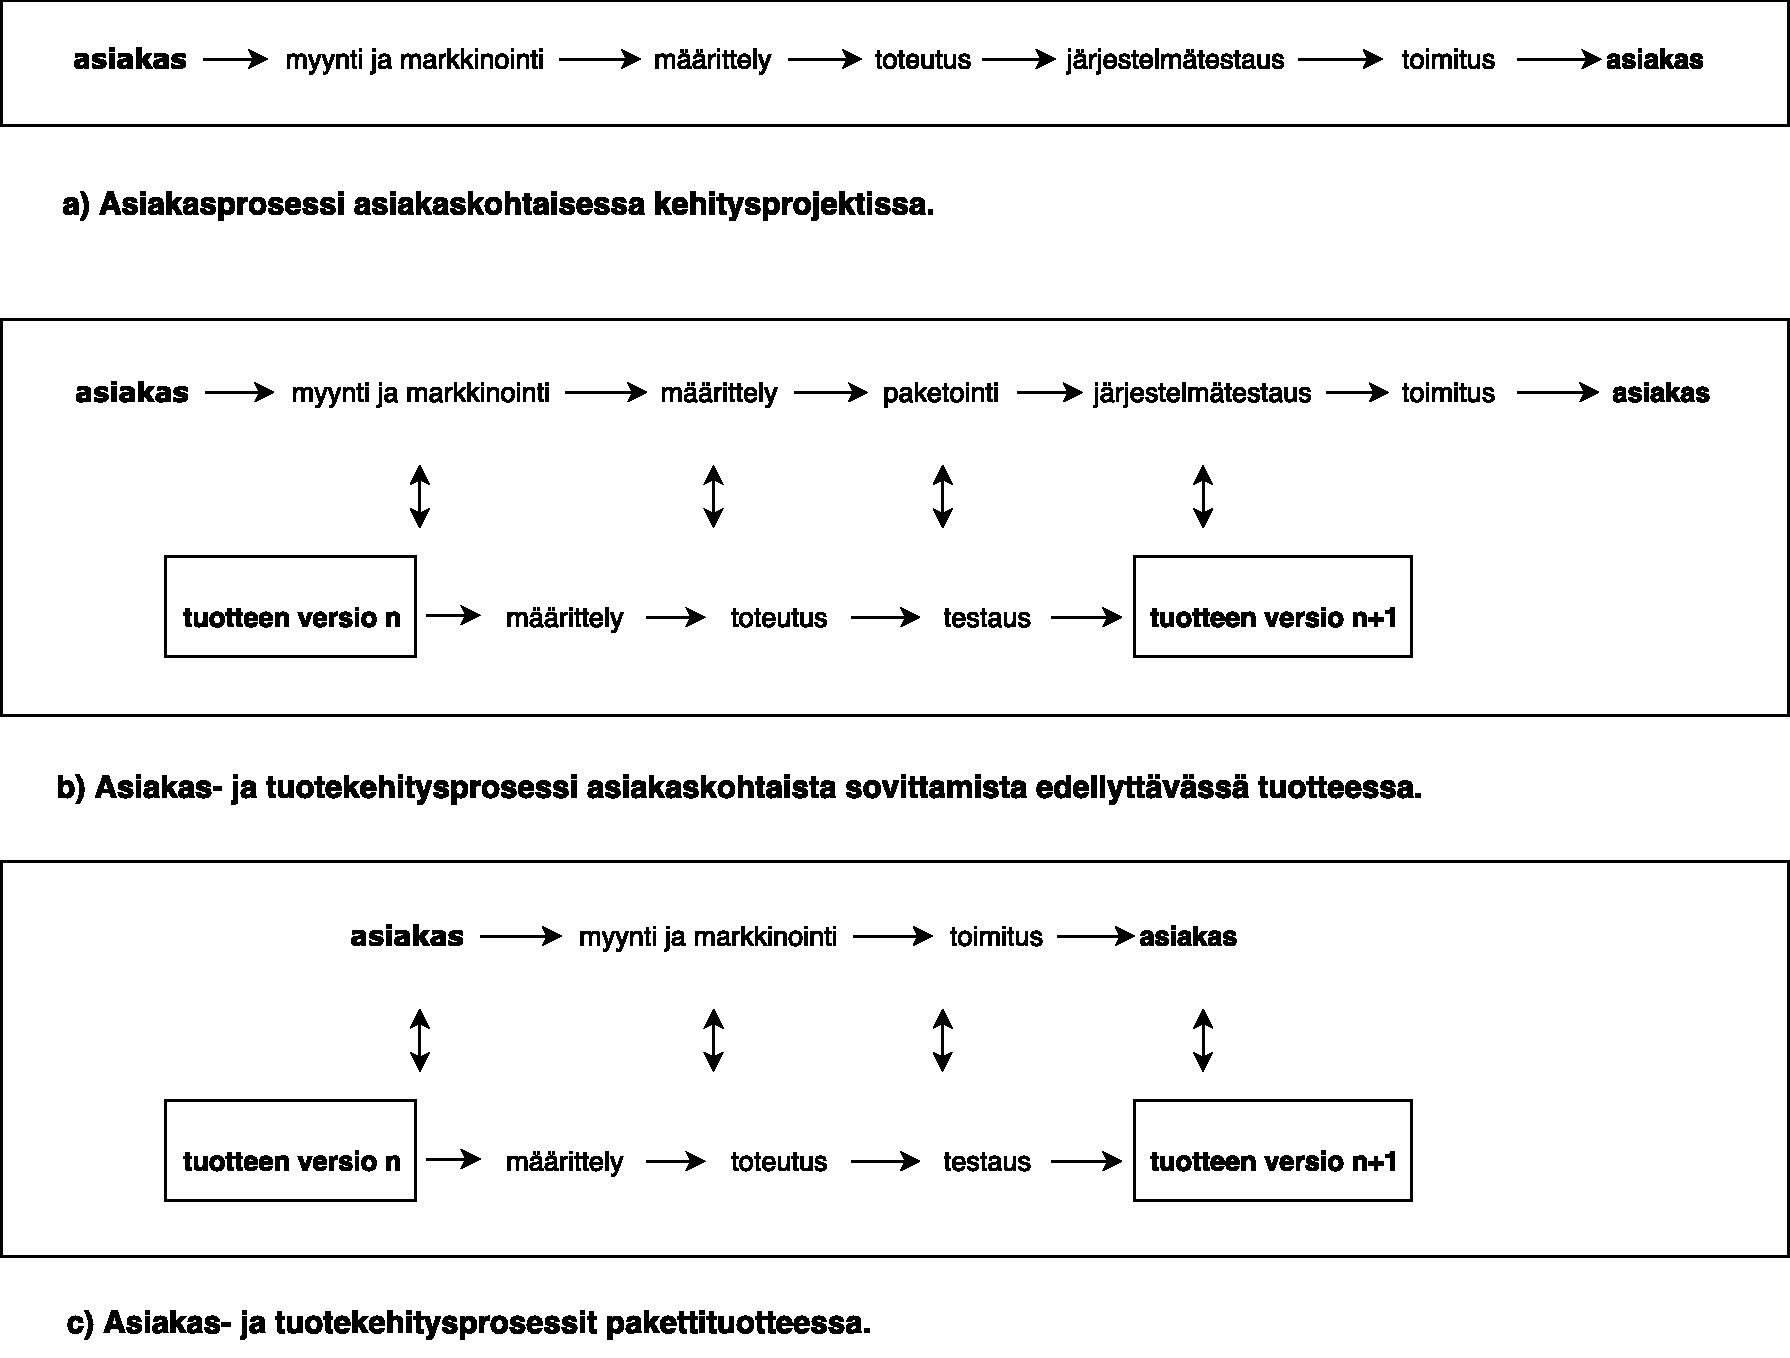
\includegraphics[scale=0.45]{asiakasprosessi.pdf}
    \caption{Asiakasprosessit eri liiketoimintamalleissa.}
    \label{fig:asiakasprosessi}
\end{figure}

On yleistä, että ohjelmistoyrityksen liiketoimintamalli sijoittuu kuvan \ref{fig:asiakasprosessi} a- ja c-kuvausten väliin. Tällöin tuotekehitys tuottaa perusmallin tuotteesta, joka paketoidaan asiakkaan toiveiden mukaan. Paketoinnilla tarkoitetaan ratkaisun kokoamista olemassa olevista komponenteista esimerkiksi konfiguroimalla. Paketointi voi myös sisältää asiakaskohtaisia muutoksia tai lisäyksiä, jolloin toiminta muuttuu asiakasprojektiksi. Yleisesti toimintaa tehostaakseen yritys pyrkii luomaan tuotteen joka on samanlainen asiakkaasta riippumatta. Usein todellisuus kuitenkin on, että asiakkaiden tarpeet vaihtelevat niin paljon, ettei asiakaskohtaiselta räätälöinniltä voi välttyä. Räätälöinnin määrää on kuitenkin hallittava, ja sen vuoksi tuotekehityksen on oltava mukana asiakasprosessissa. 

Tuotekehitysprosessi
Ylläpitoprosessi

Jos hyviä toimintamalleja ei noudateta syntyy teknistä velkaa, joka johtaa projektin loppuvaiheessa aikataulutusongelmiin.

Parempi aasinsilta:
Ohjelmistotuotannossa kuten missä tahansa toiminnassa tapahtuu inhimillisiä virheitä, mutta jos työprosesseissa ei ole virheitä mittaavaa laatukomponenttia, on riski, että virhe jää näkymättömiin ohjelmiston sisälle, ja aiheuttaa ennalta odottamattomia virhetilanteita myöhemmin tuotannossa. Tässä vaiheessa virheen korjaaminen on haastavaa jos selkeää indikaatiota virheen alkuperästä ei ole nähtävissä, ja virheen korjaavaa ohjelmistopäivitystä tai julkaisua täytyy odottaa pitkään. Aikaisemmin olikin tyypillistä nähdä ohjelmiston mukana tuleva kirjanen joka antaa ehdotuksen yleisimmistä virhetilanteista palautumiseen. Tälläiset tapaukset ovat esimerkkejä laadunvarmistuksen toimimattomuudesta jossain työprosessin vaiheessa. Hyvän laatujärjestelmän yksi tavoitteista onkin estää inhimilliä erehdyksiä. Inhimillisten erehdysten estäminen raskastekoisella ja monipuolisia laatustandardeja valvovalla prosessilla ei useinkaan ole paras ratkaisu.

Ohjelmistojen ja järjestelmien kanssa työskentelevillä ihmisillä on usein tapana suhtautua epäilevästi kankeisiin prosesseihin, ja sen johdosta ketterät menetelmät ovat kasvattaneet suosiotaan vastareaktiona kankealle prosessille. Hyvä työprosessi ohjelmistotuotannossa onkin mahdollisimman kevyt hallittavissa oleva prosessi. Ohjelmistotuotannossa hienoinkaan prosessi ei nimittäin korvaa tekijöiden ammattitaitoa. On kuitenkin täsmennettävä, että ohjemistotuotannon ammattilainen tehtävään soveltuvan prosessin kanssa päihittää aina toisen ammattilaisen, jolla ei ole hyvää prosessia. Ongelmaksi muodostuu juuri sopivan prosessin rakentaminen.

Sen vuoksi uuden prosessin rakentamista uudelleen jokaista asiakastomitusta varten tulisi välttää. Prosesseille voi toki kohdistua hyvinkin erilaisia vaatimuksia tilanteesta riippuen. Laadunhallinnan järjestelmän tulisikin tarjota valmis pohja prosessille, joka tarjoaa sopivasti taipuvan rakenteen erilaisten tavoitteiden saavuttamiseksi. Sopivan prosessin rakentaminen onkin aina kompromissi. 

Digitaalisuuden korostuessa voi harva yritys sanoa että sen liiketoimintaprosesseissa ei korostuisi tietojärjestelmien käyttö. 


Ohjelmistotuotannossa tavoitellaan ketterää, luotettavaa ja turvallista tuotetta. Kuitenkin käytännössä näiden kaikkien saavuttaminen on haastavaa. Usein tuotantoprosessia on vaikea määritellä ja mitata, jolloin prosessin hallitseminen on haastavaa. 

vaikeasti määriteltävissä olevat tuotantoprosessit, vaikeasti määriteltävissä ja mitattavissa olevan laatukomponentin puuttuminen, tuotanto- ja kehitysympäristön erot nostavat ylläpitokustannuksia 

Ohjelmistojen koko ja monimutkaisuus usein kasvavat liian nopeasti, jolloin menetetään tuotannon ketteryys. Tuotantoprosessia on vaikea määritellä ja siten mitata, koska ongelmat pyritään ratkomaan ketterästi. Joskus vaatimusmäärittelyssä ei osata kuvata todellista ongelmaa, joka halutaan ratkoa. 

Ohjelmistojen koko ja monimutkaisuus
Tuotantoprosessia vaikea määritellä ja siten mitata: prosessia on vaikea hallita, jos sitä ei voida mitata/ ohjelmistojen tekeminen on yhä liiaksi improvisointia/ liian vähän raakaa ja suoraviivaista työtä
Tuotteen määrittely on ongelmallista: asiakas ei oikein tiedä mitä haluaa/ määrittelyyn ei tunneta tieteellisiä, tai edes käytännössä hyvin toimivia menetelmiä
Tuotteen laadusta ei ole varmuutta: laadun formaali määrittely on vaikeaa/ ohjelmiston kattava testaus on käytännössä mahdotonta
Ohjelmistoa on työlästä pitää kunnossa: ylläpito = kaikki mikä tapahtuu ohjelman ensimmäisen käyttöönoton jälkeen/ kustannukset ovat huomattavasti suuremmat kuin kehityskustannukset
Projektin kulku on usein vaikeasti ennakoitavissa: projektin vaatiman työmäärän arviointi onnistuu harvoin/ teorian puuttuminen

Yleisiä ongelmia ohjelmistotuotannossa.

liiketoiminta heittää sian kehitykselle, jolloin kehitys joutuu lunastamaan lupauksen ja heittämään sian uudelleen operaatuoille. Downward spiral. Tiedä pullonkaulasi!

Ehkä jotain lisäyksiä näkymättömästä luonteesta, josta on hyvä jatkaa seuraavassa kappaleessa. Esim. sen vuoksi on tärkeää kuvata prosessit mahdollisimman tarkasti?

\subsubsection{Asiakasprosessin kehittäminen ja automatisoiminen}

separate man from machine. https://www.lean.org/balle/DisplayObject.cfm?o=3161 
Toimintojen jakamiseen liittyvät suunnittelupäätökset määrittävät, missä määrin annettu työ, tehtävä, toiminta tai vastuu on automatisoitu, ja missä määrin ne on annettu ihmisen suoritettavaksi... (iso..)

Tiedätkö mitä työ on? kuuntele se kohta.

Aloita manufacturing jne. 
insinöörit eri aloilta ovat hiljalleen kypsyneet tuntemaan oman työnsä sisällön. Devops handbook foreword!

Sen automatisoimisella saavutetaan three ways hyödyt. limit waste etc

Excessive automation: Rather than eliminating or at least simplifying
wasteful processes, they are often automated, creating additional
layers of system complexity and increasing total cost of ownership.


When kaizen teams perform value stream mapping, they often discover
that over 95 percent of the time, no value is added to products and services
as they move through the value stream. Information waste* is frequently
discovered to be a major cause. While some complexity is inherent to the
nature of business processes, much complexity is unnecessary and selfimposed.
We believe much of the unnecessary complexity is an outcome of
the reengineering trend of the 1990s. While significant productivity gains
were achieved during this period, the relentless pursuit of hyper-efficiency
and automation in some cases introduced overdesign and over-processing.
Aggressively pursuing automation limited flexibility and ability to change.
Over time, new products, services, and their supporting systems generated
a seemingly endless collection of intricately interwoven processes and
software, resulting in layers of non-value-adding activity. The psychological
inertia that was created remains very strong and resistant to change.
For example, during a kaizen project to improve information flow, one (Lean IT, 2010)

A holistic enterprise process viewpoint is not easily achieved, due to
the multidimensional nature of enterprise value streams and supporting
processes, shared services, projects, resources, and stakeholders.
However, if an organization is unable to identify its value streams, its
supporting processes, and their interrelationships, it will be unable to
make valid fact-based prioritization decisions on process improvements
and IT investments. 

Business process Management

Bussiness Process Re-Engineering

Lean



DevOps
\subsubsection{Automaatio asiakasprosessissa}
https://devops.com/automation-versus-orchestration/ 
Se että ODI-prosessi on automaattinen tarkoittaa että se rakennetaan komponenteista joihin automaatio on rakennettu sisään. Esim. onko order-prosessi rakennettu automaatio laatukomponentti mielessä? Onko toimitusprosessi rakennettu automaatio mielessä? Onko laskutusprosessi rakennettu automaatio mielessä?
Onko meidän henkilökunta tilausten vastaanotossa 

Koska Amazonilla ei ollut logistiikkaosaamista tai olemassaolevaa rakennetta, se joutui löytämään reitin muulla tavoin, verkkokauppana jossa niitä ei tarvittu. Rakentamaan disruptiivisen ominaisuuden prosesseihinsa.

Kaikki esim 2-3-tason tyypit ovat vanhaa maailmaa, jonka läsnäolo ei auta näkemään mitä voisimme tehdä jos olisi pakko. Voisimmeko ulkoistaa toimitukset Zylincille kokonaan?

Mistä työstä asiakasprosessi pääasiassa koostuu ohjelmistotuotannossa. Esimerkiksi mitkä ovat yleisiä kohtia johon uppoaa paljon työtunteja ja resursseja, mutta eivät tuota suurta arvoa? Esim infrastructure as a code.





\subsection{Asiakaspalvelujärjestelmät}

Asiakaspalvelujärjestelmä ovat organisaation keskitetty toiminto, jossa käsitellään usein suurta määrää asiakkaan yhteydenottoja. Perinteisesti tärkeitä toimintoja ovat sisääntulevat ja ulos lähtevät kontaktit. Sisään tuleva liikenne on usein asiakaspalvelua ja ulospäin lähtevä liikenne proaktiivista asikaspalvelua tai myyntiä. Asiakaspalvelujärjestelmään kuitenkin keskittyy myös muita kanavia kuten sähköposti, chat ja sosiaalinen media.

Asiakaspalvelujärjestelmän käyttäjää kutsutaan agentiksi. Agentti tarvitsee useissa tapauksissa edelleen fyysisen puhelimen ja työaseman, joskin useat uudet ratkaisut pyrkivät välttämään tarvetta tälle. Agenttien on pystyttävä ratkaisemaan asiakkaiden ongelma, ja siksi onkin järkevää, että agenteilla on erilaisia taitoja, joiden perusteella asiakaskontaktit ohjautuvat heille. Nykyään on myös tavallista, että organisaatioilla ei ole erikseen suurta asiakaspalveluorganisaatiota, ja yhä useampi työntekijä kuitenkin käyttää asiakaspalvelujärjestelmää agenttina. 

Multitentant single tenant juttua cc-järjestelmistä.

\subsection{Automaatio digitaalisessa transformaatiossa}
Kerro tässä kappaleessa miksi nyt ollaan tässä tilanteessa Telialla, että tässä yksikössä halutaan automatisoida Kontakti L:n asiakasprosessi. Miksi prosesseja pitää nyt automatisoida että voi säilyä kilpailukykyisenä? Koska DT mahdollistavat sen, ja kilpailijat yrittävät samaa, 

Digitaalisten teknologioiden hyödyntäminen yrityksen liiketoimintaprosessissa alentaa liiketominnan käyttökustannuksia ja parantaa asiakaskokemusta  \citep{lamoureux, jungner}. Lamourexin mukaan yritykset, jotka omaksuvat uusien digitaalisten teknologioiden käytön liiketoiminnassaan, suoriutuvat markkinoilla kilpailijoitaan paremmin. Hän lisää, että digitaalinen transformaatio on yrityksille selviytymisen edellytys, ja kilpailukyky markkinoilla rakentuu relevanttien teknologioiden ja niiden mahdollistamien liiketoimintavalmiuksien tunnistamiseen ja rakentamiseen. 

Digitaalisuus ja siihen liittyvä automaatio ja robotiikka ovat termeinä haastavia, koska niiden merkitys vaihtuu ajan kuluessa, eri ympäristössä ja yksilöiden mielissä. Ne myös kuvaavat monimutkaisia teknologisia edistysaskelia, joita on vaikea kuvata tyhjentävästi. Keskustelussa termit myös yksinkertaistuvat ja sekoittuvat toisiinsa. Onkin tärkeä muistaa, että juuri nyt niillä tarkoitetaan asioiden tekemistä aivan uudella tavalla, eikä vain automaation tai muun uuden teknologian käyttämistä nykyisissä prosesseissa. Mooren \citeyearpar{susanmoore} mukaan kyse on uuden arvon luomisesta, eikä vain parannuksista vanhaan. Hän täsmentää, että automaatio ei vähennä ihmistyön määrää, vaan ihmistyö kohdentuu luovien ratkaisujen tekemiseen teknologian avulla. Teknologia valjastetaan luomaan yksilöllistä arvoa ihmisille \citep{jungner, susanmoore}.

Digitaalisuus itsessään ei ole mikään uusi asia. Digitaalisten teknologioiden kehitys alkoi tietokoneen keksimisestä ja yleistymisestä. Internetin myötä tietokoneet ovat yhteydessä toisiinsa ja näin tieto on tarjolla paikasta ja ajasta riippumatta. Pilviteknologioiden myötä on mahdollista käyttää lähes rajaton määrä laskentatehoa ja tallennustilaa. Tietoliikenneyhteyksien kehittymisen myötä tietoa on mahdollista siirtää paikasta toiseen yhä nopeammin. Se mitä digitaalinen tarkoittaa, muuttuu edelleen kun aikaa kuluu. Tässä työssä digitaalisilla teknologioilla tarkoitetaan nimenomaan pilvestä saatavilla olevaa laskenta- ja tallennuskapasiteettia, sekä Internet-teknologioita, joiden avulla tietokoneet ovat yhteydessä toisiinsa. Tämä digitaalisuuden aalto on hyödyllinen monilla tavoin. 

Jungnerin \citeyearpar{jungner} mukaan hyötynä digitaalisuudessa on reaalimaailman asian muuttuminen tietokoneen ymmärtämään binäärimuotoon, jolloin tietokoneen laskentatehoa ja tallennustilaa voidaan käyttää todellisen maailman ilmiöiden seuraamiseen, ymmärtämiseen ja synnyttämiseen. Tällöin voidaan rakentaa työvälineitä mallintamaan reaalimaailman ilmiöitä tietokoneen maailmaan, siirtää reaalimaailman vuorovaikutusta tietokoneiden maailmaan ja avata tietokoneille tie toimia suoraan reaalimaailmassa. Teknologian kehitys mahdollistaa uusien toimintamallien syntymisen, joiden avulla yhä monimutkaisempia reaalimaailman asioita voidaan mallintaa tietokoneelle.

\subsubsection{Digitaalinen visio}

Lamourex \citeyearpar{lamoureux} kertoo, että yritys voi hyödyntää digitaalisen teknologian työvälineitä kehittääkseen tuotteita ja palveluita, tehokkaampia prosesseja ja asiakaskokemusta. Hänen mukaansa digitaalinen transformaatio tarkoittaa kaikkien näiden komponenttien muuttamista suurilta osin digitaalisiksi. Tällöin itse tuote tai palvelu on virtuaalinen, se ostetaan virtuaalisesta kanavasta jolloin koko asiakaspolku on virtuaalinen. 

Transformaation vaatimuksena onkin reaalimaailman toimenpiteen arvoa tuottavan osan muuntaminen tietokoneen luettavaksi ja arvotuotannon kehittäminen digitaalisessa maailman ehdoilla. Tämä vaatiikin reaalimaailmassa olevien toimintamallien pilkkomista, uudelleen järjestämistä ja karsimista \citep{leanit}. Suurin este transformaatiossa onkin organisaation vakiintunut tapa toimia, jolloin kulttuuriset näkymättömät tavat eivät sovellu digitaaliseen maailmaan \citep{jungner, lamoureux}.

Jungner \citeyearpar{jungner} kertoo tietokoneiden roolin korostuvan reaalimaailmassa, joka johtaa tehokkaampaan tapaan toimia. Monenlainen toiminta siirtyy tietokoneen suoritettavaksi. Tämän myötä kokonaiset toimialat uudistuvat ja myös koko yhteiskunta. Jungner käyttää esimerkkinä pankkialaa, joka käy läpi suurta muutosta, jossa palveluiden ylläpitäminen vaatii murto-osan siitä työvoimasta mitä aikaisemmin tarvittiin. Toisaalta pankkipalvelut ovat laajempia kuin aikaisemmin. Jungner alleviivaakin, että ei-digitaalisella tavalla toimiessa nykyinen pankkitoiminta vaatisi koko Suomen kansan työpanoksen. Lamourex \citeyearpar{lamoureux} korostaa, että
uusien teknologioiden hyödyntäminen ei ole vaihtoehto, vaan selviytymisen edellytys.

Jungner \citeyearpar{jungner} puhuu talouden ekosysteemin luovan tuhon kiihtymisestä nopeutuvan digitaalisuuden vuoksi, jossa vanhat yritykset, tuotteet, palvelut, tavat ja ammatit häviävät uusien tuottavampien sovellusten tieltä. Uusissa ammateissa työtavat muuttuvat hyödyntämään verkostoneituneita työvälineitä, ja tiedon hyödyntäminen tehostuu, jolloin innovaatioiden sykli nopeutuu. 

Lamourexin \citeyearpar{lamoureux} mukaan digitaalisten teknologioiden hienostuneisuus ja lukumäärä kasvaa innovaatioiden syklin nopeuduttua. Tämän myötä myös käyttötavat moninkertaistuvat. Uusien teknologioiden ja niiden käyttötapojen tehokkaalla hyödyntämisellä on mahdollista saada aikaan yhä isompia tuloksia. Pienikin toimija voi vallata siivun markkinasta isolta toimijalta tehokkaasti kohdennetulla ja ketterällä ratkaisulla. Lamourex \citeyearpar{lamoureux} puhuu disruptoinnista, jossa haastetaan vallitseva tila uudella radikaalilla tavalla, joka tuhoaa vanhaa ja luo uutta nopeasti. Hän tuo vahvasti esiin, että disruptointi ei ole vain pienten ja ketterien organisaatioiden yksinoikeus, sillä myös suuryritys voi disruptoida markkinoita. Usein suuryrityksellä onkin etulyöntiasema olemassaolevien prosessien muodossa. Kokeilujen aloittamista tai onnistumista kuitenkin usein heikentää selkeän vision puuttuminen uusien teknologioiden hyödyntämisestä, missä nopea kokeilu on valttia. Lamourex tarjoaa tähän jatkuvan korkean tason viitekehyksen toimintamallina digitaalisen teknologian hyödyntämiseen.



mutta kokeiluja estää selkeän vision puuttuminen uusien teknologioiden hyötyjen tunnistamisessa.

Lopeta kappale siihen että viahtoehtoja ei juuri ole jos tulevaisuudessa haluaa olla olemassa.


tieto lähteä kokeilemaan rohkeasti uusia ideoita, mutta ilman selkeää visiota uusien teknologioiden käytöstä, ei hyödyt kotiudu koskaan. 

Disruptointi ei kuitenkaan ole vain pienten ja ketterien toimijoiden etuoikeus, vaan isolla toimijalla on jopa paremmat edellytykset disruptointiin. Se kuitenkin vaatii kulttuuria joissa uusia villejä kokeiluja on mahdollista tehdä jatkuvalla syötöllä, mutta silti harkiten. Iso toimija joka pystyy nopeuttamaan omaa arvotuotannon sykliä hyädyntämällä digitaalisia teknologioita hallitsee digitaalisuuden seuraavaa aikakautta. Perässä hiihtäminenkään ei ole kannattavaa sillä yriksen olemassaolon edellytys tulee digitaalisen maailman kautta. Olemassaolo on mahdollista vain käyttämällä digitaalisia teknologioita liiketoiminnassa, mutta oikeasti kilpaileminen vaatii kykyä nopeuttaa innovaatiosykliä riittävästi.





Transformaatio onkin monen yrityksen listalla kärkihankkeena jne.

jatka tästä<


Operaattorin näkökulmasta digitalissaa



Yrityksen näkökulmasta teknologialla parannetaan tuotteita, sisäisiä prosesseja ja asiakaskokemusta. Pelkästään teknologian käyttäminen ei kuitenkaan tuo hyötyä liiketoimintaan. Valitulla teknologialla täytyy olla potentiaalia kasvattaa kilpailukykyä määrätyssä aikajaksossa, ja investoinnin tulee ottaa riskit huomioon. Uusia teknologioita tulee ja menee, ja siksi tulisikin olla kykyjä tutkia useampia potentiaalisia teknologioita saman aikaisesti. Ajankohdan tulee myös olla sopiva, koska teknologiat saattavat vanhentua luultua nopeammin ja liian aikaisin tehty investointi uuteen teknologiaan saattaa heikentää kilpailuedun saamista. Teknologian hyödyntämisessä vaaditaan myös selkeä kuva liiketoimintavalmiudesta joka halutaan rakentaa sen avulla. Uusien teknologioiden käytön omaksuminen liiketoiminnan tavoitteiden saavuttamiseksi ei myöskään tapahdu itsestään. Teknologian käyttäminen kilpailuedun saavuttamiseksi markkinoilla onkin organisaation opittu taito. Eli organisaation sisäisten ja ulkoisten tavoitteen kannalta relevanttien sidosryhmien kyky tehdä yhteistyötä. Tämän kyky on vaikeampi rakentaa organisaatioissa, joissa tavoitteen kannalta relevantteja sidosryhmiä on useampia. Suurempi sidosryhmien määrä vaikeuttaa tiedon vaihtamista ja kommunikointia. Uuden teknologian hyödyntäminen kilpailiedun saavuttamiseksi vaatiikin toimintamallin muuttumista, usein yksinkertaisempaan suuntaan.





Digitaalisen teknologian myötä automaatio on scriptausta apeja jne pilvessä jne. Jungner puhui kaikki on avointa



Digitalisaation työkalupakki(aoit, rpa, ...)
Digitalisaation menetelmät (devops, lean, kaikki on avointa...)
Muutosvoimat operaattorin näkökulmasta(doing digital right)
Telain strategia vastaamaan muutosvoimiin
Muutosvoimat
multi single?
Telian/operaattoreiden haasteet muutosvoimissa
- Teknologian keihäänkärjet, order to cash
Ratkaisuja tarjoavat 

teollisuudessa disruptioitiin ja sitten lähti muutos leaniin.
Automaatio ja DevOps tulee täällä. Tämän vuoksi jne.

Multi-single asiaa myös

\citep{lamoureux}

\begin{itemize}
\item[--]Amazon-Wallmart(Disruptor-Disrupted): Wallmart mastered cost management, supply chain efficiency & merchandising. Amazon became more valuable in just 21 years from nothing! Amazon entered mature industry, and used viable digital tech to make their processes efficient & customer buying process easy. Walmart had advantage from beginning but did not embrace digitality into its processes. Can today’s established businesses leverage digital tech to be the disruptor, not the disrupted. Existing businesses that leverage their relationships  and processes and energetically apply new, viable technologies will win.
\item[--]New technologies have become more viable to enable more efficient processes and facilitation of the customer journey, like cloud technologies for computer service or RPA 
\item[--]\citep{lamoureux}
Jatkuva viitekehys digitaalisuuteen:
Digitaaliset teknologiat - liiketoiminnallinen käyttökohde - Liiketoiminnan tulos
\item[--]\citep{lamoureux}.
Teknologioiden määrä ja kompleksisuus kasvaa eksponentiaalisesti. Johtajat tietävät että heidän täytyy investoida uusiin teknologioihin, mutta rajallisilla resursseilla operoidessa täytyy arvioida mahdollisia tuottoja joita teknologioiden hyödyntämisessä on mahdollista saavuttaa, koska se raha on pois ns. perinteisen liiketoiminnan pyörittämisestä.
\item[--]Kolme aikakautta:
1950-2000  Alkoi kun yritykset aloittivat automatisoinnin. Yritykset rakensivat omia ohjelmistoja aluksi, kaupalliset tuotteet tulivat 70-luvulla, PC:t 80-luvulla, Internet 90-luvulla, mutta se muutti asioita vasta 2000-luvulla.
\item[--]Typical automation: hallinta ja vaihdantaprosessit kuten palkanlaskenta, tuotanto, toimitus, tilaustenhallinta, saatavien hallinta, taloushallinto. Tietoa hallittiin lokaalisti lähellä sen lähdettä. 
Liiketoimintaan vaikuttavat tu
\item[--]2000-2015 Alkoi Internetin yleistymisen myötä. 
\end{itemize}




\subsection{Kappaleen yhteenveto}


Ydinprosessit Telialla ja ODI prosessi niiden joukossa. Minkälaista tehtävää se suorittaa?










\clearpage

\section{Tutkimusaineisto ja -menetelmät}
%\section{Materials and methods}

ODI-prosessi koostuu osaprosesseista ja niiden komponenteista. Mihin laatuvaatimuksiin nykyiset komponentit ovat rakennettu?



MIssä liiketominta casessa automaatiota tulisi hyödyntää. 

Tutki miten ODI-prosessi rakennetaan Telialla juuri nyt.

Tutki valmiita komponentteja ja kun niitä yhdistellään tutki mahdollisia manuaalisia työvaiheita jotka ovat riski.

Koko business case asiaakspalvelujärjestelmätoimituksissa.

Tässä osassa kuvataan käytetty tutkimusaineisto ja
tutkimuksen metodologiset valinnat, sekä
kerrotaan tutkimuksen toteutustapa ja käytetyt menetelmät. 

\clearpage

\section{Tulokset}
%\section{Results}
Miten ODI-prosessi rakennetaan Telialla???
Nykyinen laatujärjestelmä ODI-prosessin tekemiseen ei ole määritelty, vaan tuotepäälliköiden päässä.
Laatujärjestelmä on ODi-labraus. Miten se vastaa laatumittauksesta?

Pitää osata tuotteistaa jotain sellaista joka vastaa asiakastarvetta ja kun siitä saadaan kokemusta lyhenee läpimeno ja opitaan mestareiksi tehostamisessa. Tämän jälkeen voidaan sanoa mitä kannattaa automatisoida. Siihen robotisaatiomalliin on saatava vihreät valot. Eli on osattava vastata kysymyksiin tarkasti!


Tässä osassa esitetään tulokset ja vastataan tutkielman alussa
esitettyihin tutkimuskysymyksiin. Tieteellisen kirjoitelman
arvo mitataan tässä osassa esitettyjen tulosten perusteella. 

%% Huomaa seuraavassa kappaleessa lainausmerkkien ulkopuolella piste, 
%% koska piste ei lopeta lainattua tekstinpätkää.
%% Jos lainattu tekstinpätkä loppuu välimerkkiin, tulee välimerkki
%% lainausmerkkien sisälle: 
%% "Et tu, Brute?" sanoi Caesar kuollessaan.
Tutkimustuloksien merkitystä on aina syytä arvioida ja tarkastella
kriittisesti.  Joskus tarkastelu voi olla tässä osassa, mutta se
voidaan myös jättää viimeiseen osaan, jolloin viimeisen osan nimeksi
tulee >>Tarkastelu>>. Tutkimustulosten merkitystä voi arvioida myös
>>Johtopäätökset>>-otsikon alla viimeisessä osassa. 

Tässä osassa on syytä myös arvioida tutkimustulosten luotettavuutta.
Jos tutkimustulosten merkitystä arvioidaan >>Tarkastelu>>-osassa,
voi luotettavuuden arviointi olla myös siellä. 

\clearpage

\section{Yhteenveto}
%\section{Summary} 

Opinnäytteen tekijä vastaa siitä, että opinnäyte on tässä dokumentissa
ja opinnäytteen tekemistä käsittelevillä luennoilla sekä
harjoituksissa annettujen ohjeiden mukainen muotoseikoiltaan,
rakenteeltaan ja ulkoasultaan.



\clearpage
%% Lähdeluettelo
%%
%% \phantomsection varmistaa, että hyperref-paketti latoo hypertekstilinkit
%% oikein.
%%
%% The \phantomsection command is nessesary for hyperref to jump to the 
%% correct page, in other words it puts a hyper marker on the page.

\phantomsection
%\addcontentsline{toc}{section}{Viitteet}
%\addcontentsline{toc}{section}{References}
%%\begin{thebibliography}{99}
\bibliography{lahteet}

%% Alla pilkun jälkeen on pakotettu oikea väli \<välilyönti>-merkeillä.

%%\end{thebibliography}

%% Liitteet 
\appendix 
\clearpage
%% Lisää tekstin "Liitteet" sisällysluetteloon
%%
%% Adds the word "Appendices" to the table of contents
\addtocontents{toc}{\protect\contentsline{section}{Liiteet}{}{appendix}}
%\addtocontents{toc}{\protect\contentsline{section}{Appendices}{}{appendix}}

\section{Esimerkki liitteestä\label{LiiteA}}
%% Liitteiden kaavat, taulukot ja kuvat numeroidaan omana kokonaisuutenaan
%%
%% Equations, tables and figures have their own numbering in Appendices
\renewcommand{\theequation}{A\arabic{equation}}
\setcounter{equation}{0}  
\renewcommand{\thefigure}{A\arabic{figure}}
\setcounter{figure}{0}
\renewcommand{\thetable}{A\arabic{table}}
\setcounter{table}{0}

Liitteet eivät ole opinnäytteen kannalta välttämättömiä ja 
opinnäytteen tekijän on 
kirjoittamaan ryhtyessään hyvä ajatella pärjäävänsä ilman liitteitä.
Kokemattomat kirjoittajat, jotka ovat huolissaan
tekstiosan pituudesta, paisuttavat turhan 
helposti liitteitä pitääkseen tekstiosan pituuden annetuissa rajoissa.
Tällä tavalla ei synny hyvää opinnäytettä.   

Liite on itsenäinen kokonaisuus, vaikka se täydentääkin tekstiosaa.
Liite ei siten ole pelkkä listaus, kuva tai taulukko, vaan 
liitteessä selitetään aina sisällön laatu ja tarkoitus. 

Liitteeseen voi laittaa esimerkiksi listauksia. Alla on 
listausesimerkki tämän liitteen luomisesta. 

%% Verbatim-ympäristö ei muotoile tai tavuta tekstiä. Fontti on monospace.
%% Verbatim-ympäristön sisällä annettuja komentoja ei LaTeX käsittele. 
%% Vasta \end{verbatim}-komennon jälkeen jatketaan käsittelyä.
\begin{verbatim}
	\clearpage
	\appendix
	\addcontentsline{toc}{section}{Liite A}
	\section*{Liite A}
	...
	\thispagestyle{empty}
	...
	tekstiä
	...
	\clearpage
\end{verbatim}

Kaavojen numerointi muodostaa liitteissä oman kokonaisuutensa:
\begin{eqnarray}
d \wedge A  &=& F, \label{liitekaava1}\\
d \wedge F  &=& 0. \label{liitekaava2}
\end{eqnarray}


\clearpage
\section{Toinen esimerkki liitteestä\label{LiiteB}}

%% Liitteiden kaavat, taulukot ja kuvat numeroidaan omana kokonaisuutenaan
%%
%% Equations, tables and figures have their own numbering in Appendices
\renewcommand{\theequation}{B\arabic{equation}}
\setcounter{equation}{0}  
\renewcommand{\thefigure}{B\arabic{figure}}
\setcounter{figure}{0}
\renewcommand{\thetable}{B\arabic{table}}
\setcounter{table}{0}

Liitteissä voi myös olla kuvia, jotka
eivät sovi leipätekstin joukkoon:
%% Ympäristön figure parametrit htb pakottavat
%% kuvan tähän, eikä LaTeX yritä siirrellä niitä
%% hyväksi katsomaansa paikkaan. 
%% Ympäristöä center voi käyttää \centering-
%% komennon sijaan
%%
%% Example of a figure, note the use of htb parameters which force
%% the figure to be inserted here
\begin{figure}[htb]
\begin{center}
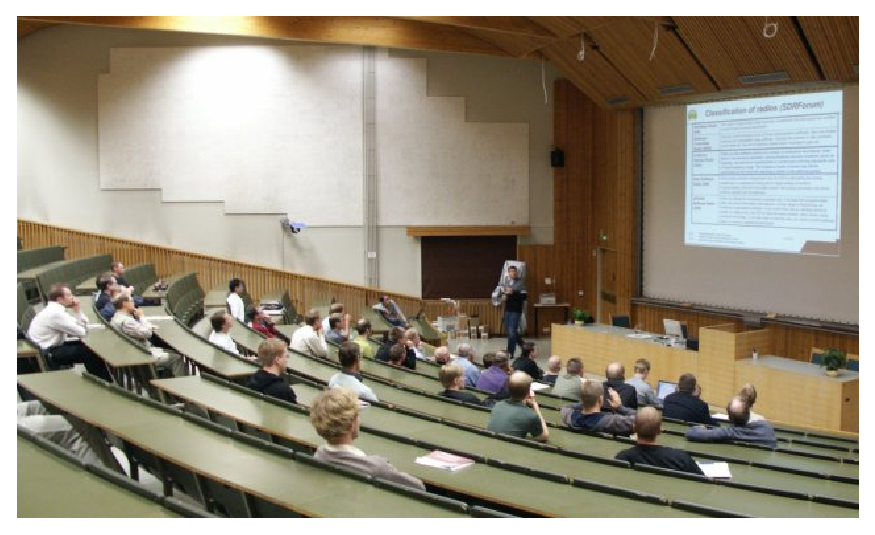
\includegraphics[height=8cm]{kuva2}
\end{center}
\caption{Kuvateksti, jossa on liitteen numerointi \label{liitekuva}}
\end{figure}
%%
Liitteiden taulukoiden numerointi on kuvien ja kaavojen kaltainen:
\begin{table}[htb]
\caption{Taulukon kuvateksti. \label{liitetaulukko}}
\begin{center}
\fbox{
\begin{tabular}{lp{0.5\linewidth}}
9.00--9.55  & Käytettävyystestauksen tiedotustilaisuus (osanottajat
ovat saaneet sähköpostitse valmistautumistehtävät, joten tiedotustilaisuus
voidaan pitää lyhyenä).\\
9.55--10.00 & Testausalueelle siirtyminen
\end{tabular}}
\end{center}
\end{table}
Kaavojen numerointi muodostaa liitteissä oman kokonaisuutensa:
\begin{eqnarray}
T_{ik} &=& -p g_{ik} + w u_i u_k + \tau_{ik},  \label{liitekaava3} \\
n_i    &=& n u_i + v_i.                        \label{liitekaava4}
\end{eqnarray}

\end{document}
